\section{Quantifier Elimination with the Virtual Substitution}
\label{sec:quantifier-elimination-with-the-virtual-substitution}
Let $\varphi$ is a quantifier-free real arithmetic formula where $x\in \varphi$ and $x$ has at most quadratic in $\varphi$. After eliminating existential and universal qualifier with virtual substitution we will get the following equivalences, respectively:
\begin{alignat}{2}
	&\exists x \varphi^\mathbb{R} \Longleftrightarrow \bigvee\limits_{t\in T(x,\varphi^\mathbb{R})}  (\varphi^\mathbb{R} [t\backslash\backslash x] \wedge C_t)\qquad   \\
	& \forall x \varphi^\mathbb{R} \Longleftrightarrow \bigwedge\limits_{t\in T(x,\varphi^\mathbb{R})}  (C_{t}\rightarrow\varphi^\mathbb{R} [t\backslash\backslash x] )\qquad
\end{alignat}

Now, let us consider $\exists y\exists x\varphi$ where, $\varphi = (x^{2}y + x + y = 0) \wedge (y^{2} -2 < 0)$. We already constructed all the test candidates for $x$ and $y$ in all the polynomials of $\varphi$. Also we get to know about virtual substitution rules. Based on virtual substitution rules, we can eliminate all occurrences of $x$ and $y$ from $\varphi$ by successively eliminating all bound variables ($x,y$) starting with the inner most one.
\begin{center}
	\input{ro_4.tex}
\end{center}
The solution values for $x$ and $y$ in $\varphi$ is shown in the figure \ref{fig:ro_1} and \ref{fig:ro_4}. Also Figure\ref{fig:graph} illustrates an overview of solving non-linear real arithmetic formula with virtual substitution.
\begin{figure}[htb] % where to insert the figure: h=here, t=top, b=bottom,
	% the order htb shows which position is preffered
	\begin{center}
	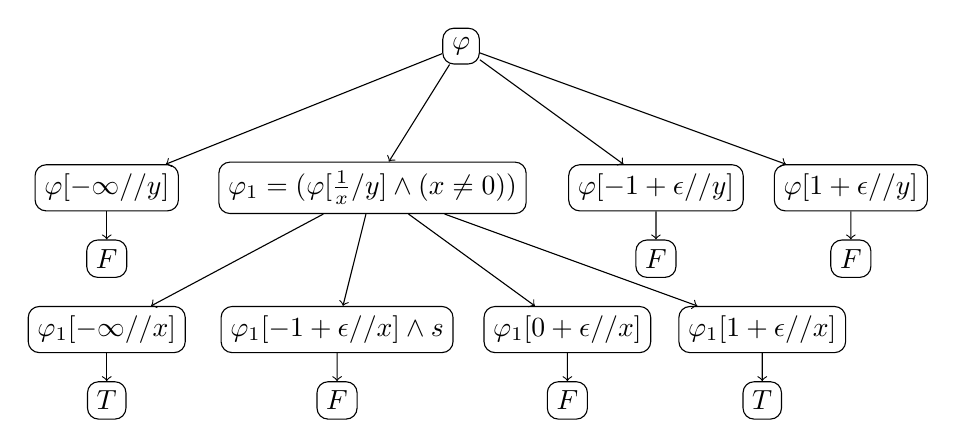
\begin{tikzpicture}[scale=0.9, 
				    state/.style={draw, rounded corners, fill=none,
				    			  text centered, text=black}]
	\node[state] (u1) at (5, 7) {$\varphi$};
	\node[state] (u2) at (0, 5) {$\varphi[-\infty//y]$};
	\node[state] (u3) at (3.75, 5) {$\varphi_{1}=(\varphi[\frac{1}{x}/y]\wedge (x\neq0))$};
	\node[state] (u4) at (7.75, 5) {$\varphi[-1+\epsilon//y]$};
	\node[state] (u5) at (0, 4) {$F$};
	\node[state] (u6) at (10.5, 5) {$\varphi[1+\epsilon//y]$};
	\node[state] (u7) at (0, 3) {$\varphi_{1}[-\infty//x]$};
	\node[state] (u8) at (3.25, 3) {$\varphi_{1}[-1+\epsilon//x] \wedge s$};
	\node[state] (u9) at (6.5, 3) {$\varphi_{1}[0+\epsilon//x]$};
	\node[state] (u15) at (9.25, 3) {$\varphi_{1}[1+\epsilon//x]$};
	\node[state] (u10) at (7.75, 4) {$F$};
	\node[state] (u11) at (10.5, 4) {$F$};
	\node[state] (u12) at (0, 2) {$T$};
	\node[state] (u13) at (3.25, 2) {$F$};
	\node[state] (u14) at (6.5, 2) {$F$};
	\node[state] (u16) at (9.25, 2) {$T$};
	
	\path[->] 	(u1)  edge   (u2);
	\path[->] 	(u1)  edge   (u3);
	\path[->] 	(u1)  edge   (u4);
	\path[->] 	(u1)  edge   (u6);
	\path[->] 	(u2)  edge   (u5);
	\path[->] 	(u3)  edge   (u7);
	\path[->] 	(u3)  edge   (u8);
	\path[->] 	(u3)  edge   (u9);
	\path[->] 	(u4)  edge   (u10);
	\path[->] 	(u6)  edge   (u11);
	\path[->] 	(u8)  edge   (u13);
	\path[->] 	(u7)  edge   (u12);
	\path[->] 	(u9)  edge   (u14);
	\path[->] 	(u3)  edge   (u15);
	\path[->] 	(u15)  edge   (u16);

\end{tikzpicture}

	\end{center}
	\caption{Example of Virtual Substitution.}
	\label{fig:graph}
\end{figure}

We get the proof of equation (4.1) which we have explained throughout this paper by an example of non-linear real arithmetic formula. Equation (4.2) can be implied by equation (4.1) as follows:
%C_{\sim}(\varphi^\mathbb{R})=C_{\sim}(\neg\varphi^\mathbb{R})
\begin{alignat}{2}
	& \forall x. \varphi\qquad   
	&&\stackrel{}{\Longleftrightarrow} \neg\exists x.\neg\varphi \\
	& 
	&&\stackrel{}{\Longleftrightarrow} \neg(\bigvee\limits_{t\in T(x,\neg \varphi)}
	 (\neg\varphi [t\backslash\backslash x] \wedge C_t) \\
	& 
	&&\stackrel{}{\Longleftrightarrow} \bigwedge\limits_{t\in T(x,\neg \varphi)} (\varphi [t\backslash\backslash x] \vee\neg C_{t}) \\
	& 
	&&\stackrel{}{\Longleftrightarrow}  \bigwedge\limits_{t\in T(x, \varphi)} (C_{t} \rightarrow \varphi [t\backslash\backslash x])
\end{alignat}
where, we get 
\begin{itemize}
	\item Equation $4.4$ by Equation $4.1$.
	\item Equation $4.5$ and Equation $4.6$ after applying $\neg((\neg\varphi_{1})\wedge\varphi_{2})=(\varphi_{1} \vee \neg\varphi_{2})$ and $(\varphi_{1} \vee \neg\varphi_{2})=(\varphi_{2} \rightarrow \varphi_{1})$, respectively.
\end{itemize}